\section{Overview}\label{sec:overview}
This section describes the steps of our method on an abstract level.
\autoref{fig:process_figure} visualizes these steps as a flowchart.
The method takes a corpus as an input and produces evaluation results as output.
Each step of the method is described in later sections in more detail.

\subsection*{Step 1: Preprocessing Phase}
In this step, we apply different preprocessing methods to simplify the dataset and remove redundant information.
Details of this phase are given in \autoref{sec:prepro}.
After finishing this phase, we are left with $\sim$?? documents and $\sim$?? words to form the corpus, which will be used in future steps.

\subsection*{Step 2: \Gls{lda} Models}
In this step, we train the standard \gls{lda} model, the category, author, and taxonomy metadata models as well as the combinations of these models on the corpus.
The standard \gls{lda} model, the metadata models, and the combination models are described further in \autoref{sec:lda}, \autoref{sec:metadata}, and \autoref{sec:combinations}, respectively.
The models are trained based on topic coherence, and after the training process the models are evaluated further.

\subsection*{Step 3: Evaluation of \gls{lda} Models}
In this step, we setup an experiment to evaluate the topic models trained in the previous step.
The evaluation metrics chosen for the experiment are perplexity and topic coherence.
Along with these evaluation metrics, human evaluation of the topics generated is also done to get a deeper understanding of what the models learn.
The experiment and results are presented in \autoref{sec:experiment} and are analyzed and discussed in \autoref{sec:discussion}.

\todo[inline]{Change/add more to the section as we figure out specifically what we do.}

\tikzstyle{process} = [rectangle, rounded corners, minimum width=2cm, minimum height=1cm,text centered, draw=black, fill=gray!50]
\tikzstyle{decision} = [diamond, minimum width=2cm, minimum height=1cm, text centered, draw=black, fill=green!30]

% one line
%\begin{figure}[ht]
%    \centering
%    \begin{tikzpicture}[node distance=2cm]
%    %\draw[step=1cm,gray,very thin] (-8,-8) grid (8,8);
%	\node (Dataset) [process] {(Input) Nordjyske Dataset};
%	\node (Cleaning)[process, below of=Dataset] {(1) Preprocessing Phase};
%	\node (Training) [process, below of=Cleaning] {(2)Train IR Methods};
%	\node (Query) [process, below of=Training] {(3) Query Generation};
%	\node (Evaluate) [process, below of=Query] {(4) Evaluate Models};
%	\node (Result) [process, below of=Evaluate] {(Output) Results};
%	\draw [->, very thick] (Dataset) edge (Cleaning); 
%	\draw [->, very thick] (Cleaning) edge (Training);
%	\draw [->, very thick] (Training) edge (Query);
%	\draw [->, very thick] (Query) edge (Evaluate);
%	\draw [->, very thick] (Evaluate) edge (Result);
%\end{tikzpicture}
%	\caption{The method visualized as a flowchart, where a dataset consisting of articles is processed into a list of ranked results.}
%    \label{fig:process_figure}
%\end{figure}

\begin{figure}[ht]
	\centering
	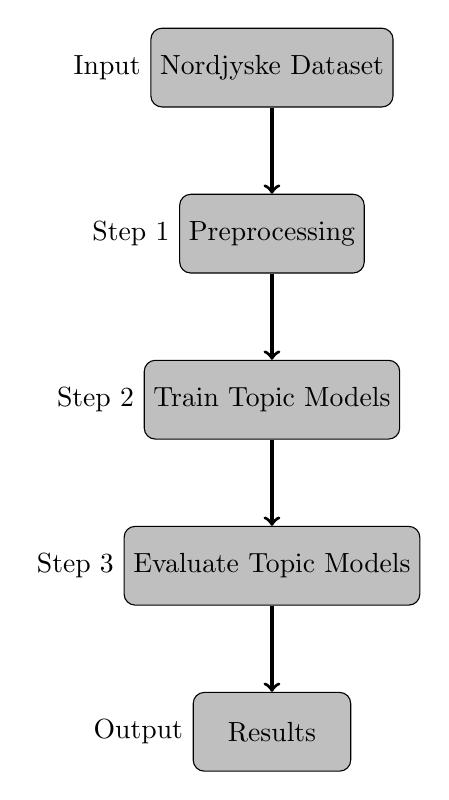
\begin{tikzpicture}[node distance=6em]
	%\draw[step=1cm,gray,very thin] (-8,-8) grid (8,8);
	\node (Dataset) [process, label=left:{Input}] {Nordjyske Dataset};
	\node (Cleaning)[process, below of=Dataset, label=left:{Step 1}] {Preprocessing};
	\node (Training) [process, below of=Cleaning, label=left:{Step 2}] {Train Topic Models};
	%\node (Query) [process, below of=Dataset, label=Step 3, yshift=2.5cm] {Query Generation};
	\node (Evaluate) [process, below of=Training, label=left:{Step 3}] {Evaluate Topic Models};
	\node (Result) [process, below of=Evaluate, label=left:{Output}] {Results};
	\draw [->, very thick] (Dataset) edge (Cleaning); 
	\draw [->, very thick] (Cleaning) edge (Training);
	\draw[->, very thick] (Training) edge (Evaluate);
	%\draw [->, very thick] (Query) edge (Evaluate);
	\draw [->, very thick] (Evaluate) edge (Result);
	\end{tikzpicture}
	\caption{The method visualized as a flowchart, where a dataset consisting of articles is processed into a list of evaluation results.}
	\label{fig:process_figure}
\end{figure}
